\documentclass[preprint,3p,11pt,sort]{elsarticle}
%DIF LATEXDIFF DIFFERENCE FILE
%DIF DEL Revisions\main_flat.tex   Fri Sep 13 21:26:25 2024
%DIF ADD main.tex                  Fri Sep 13 21:26:38 2024
\usepackage[utf8]{inputenc}

% Maths
\usepackage{amsmath,amssymb,amsfonts} % Equations
\usepackage{textcomp, gensymb} % Symbol: \degree

% Tables
\usepackage{multirow}

% Images
\usepackage{graphicx}
\usepackage{caption} % Improvements to figures, extends functionality with more options
\usepackage{placeins} % \FloatBarrier

% Text Modification
\usepackage[colorlinks=true, allcolors=blue]{hyperref} % Hyperlinks

% Figure & table ref
\newcommand{\figref}[1]{Fig.~\ref{#1}}
\newcommand{\tbref}[1]{Table~\ref{#1}}
\newcommand{\secref}[1]{Section~\ref{#1}}


%%%%%%%%%%%%%%%%%%%%%%%%%%%%%%%%%%%%%%%%%%%%%%%%%%%%%%%%%%%%%%%%%%%%%%%%%%%%%%%%%
%%%%%%%%%%%%%%%%%%%%%%%%%%%%%%%%%%%%%%%%%%%%%%%%%%%%%%%%%%%%%%%%%%%%%%%%%%%%%%%%%
\journal{JournalName}
%DIF PREAMBLE EXTENSION ADDED BY LATEXDIFF
% Brandon Changed %DIF PREAMBLE
%   Deleted=red with strike-out %DIF PREAMBLE
%   Added=blue %DIF PREAMBLE
\RequirePackage[normalem]{ulem} %DIF PREAMBLE
\RequirePackage{color} %DIF PREAMBLE
\definecolor{difRed}{RGB}{192,0,0} %DIF PREAMBLE
\definecolor{difBlue}{RGB}{0,0,192} %DIF PREAMBLE
\providecommand{\DIFaddtex}[1]{{\protect\color{difBlue}#1}} %DIF PREAMBLE
\providecommand{\DIFdeltex}[1]{{\protect\color{difRed}\sout{#1}}} %DIF PREAMBLE
%DIF SAFE PREAMBLE %DIF PREAMBLE
\providecommand{\DIFaddbegin}{} %DIF PREAMBLE
\providecommand{\DIFaddend}{} %DIF PREAMBLE
\providecommand{\DIFdelbegin}{} %DIF PREAMBLE
\providecommand{\DIFdelend}{} %DIF PREAMBLE
\providecommand{\DIFmodbegin}{} %DIF PREAMBLE
\providecommand{\DIFmodend}{} %DIF PREAMBLE
%DIF FLOATSAFE PREAMBLE %DIF PREAMBLE
\providecommand{\DIFaddFL}[1]{\DIFadd{#1}} %DIF PREAMBLE
\providecommand{\DIFdelFL}[1]{\DIFdel{#1}} %DIF PREAMBLE
\providecommand{\DIFaddbeginFL}{} %DIF PREAMBLE
\providecommand{\DIFaddendFL}{} %DIF PREAMBLE
\providecommand{\DIFdelbeginFL}{} %DIF PREAMBLE
\providecommand{\DIFdelendFL}{} %DIF PREAMBLE
%BJ:EXTRA %DIF PREAMBLE
\hypersetup{hidelinks} %BJ: Without this one can not determine what ref is added or unchanged as both would be blue %DIF PREAMBLE
%BJ:END %DIF PREAMBLE
%DIF HYPERREF PREAMBLE %DIF PREAMBLE
\providecommand{\DIFadd}[1]{\texorpdfstring{\DIFaddtex{#1}}{#1}} %DIF PREAMBLE
\providecommand{\DIFdel}[1]{\texorpdfstring{\DIFdeltex{#1}}{}} %DIF PREAMBLE
%DIF AMSMATHULEM PREAMBLE %DIF PREAMBLE
\makeatletter %DIF PREAMBLE
\let\sout@orig\sout %DIF PREAMBLE
\renewcommand{\sout}[1]{\ifmmode\text{\sout@orig{\ensuremath{#1}}}\else\sout@orig{#1}\fi} %DIF PREAMBLE
\makeatother %DIF PREAMBLE
%DIF COLORLISTINGS PREAMBLE %DIF PREAMBLE
\RequirePackage{listings} %DIF PREAMBLE
\RequirePackage{color} %DIF PREAMBLE
\lstdefinelanguage{DIFcode}{ %DIF PREAMBLE
%DIF DIFCODE_UNDERLINE %DIF PREAMBLE
  moredelim=[il][\color{red}\sout]{\%DIF\ <\ }, %DIF PREAMBLE
  moredelim=[il][\color{blue}\uwave]{\%DIF\ >\ } %DIF PREAMBLE
} %DIF PREAMBLE
\lstdefinestyle{DIFverbatimstyle}{ %DIF PREAMBLE
	language=DIFcode, %DIF PREAMBLE
	basicstyle=\ttfamily, %DIF PREAMBLE
	columns=fullflexible, %DIF PREAMBLE
	keepspaces=true %DIF PREAMBLE
} %DIF PREAMBLE
\lstnewenvironment{DIFverbatim}{\lstset{style=DIFverbatimstyle}}{} %DIF PREAMBLE
\lstnewenvironment{DIFverbatim*}{\lstset{style=DIFverbatimstyle,showspaces=true}}{} %DIF PREAMBLE
\lstset{extendedchars=\true,inputencoding=utf8}

%DIF END PREAMBLE EXTENSION ADDED BY LATEXDIFF

\begin{document}
\begin{frontmatter}

\title{My Example Manuscript  \DIFadd{is Great} }

 %DIFDELCMD < \nonumnote{Abbreviations: aaa}
%DIFDELCMD < %%%
  \nonumnote{Abbreviations: section (sec), sub-section (ssec)}
 

\begin{abstract}
    This is an example manuscript. It showcases a few common latex features so that I can show how latexdiff  \DIFdel{interacts }  \DIFadd{and the powershell scripts interact } with them.
\end{abstract}

\begin{keyword}
    a \sep b \sep c \sep d  \sep \DIFadd{e
} \end{keyword}

\end{frontmatter}

%%%%%%%%%%%%%%%%%%%%%%%%%%%%%%%%%%%%%%%%%%%%%%%%%%%%%%%%%%%%%%%%%%%%%%%%%%%%%%%%%
%%%%%%%%%%%%%%%%%%%%%%%%%%%%%%%%%%%%%%%%%%%%%%%%%%%%%%%%%%%%%%%%%%%%%%%%%%%%%%%%%
\section{Introduction} \label{sec:intro}
This is an example manuscript.

The structure of this article is as follows: \secref{sec:mySection} showcases the use of SSSSR sections. \secref{sec:ContentTypes} shows how to display many different types of content.


%%%%%%%%%%%%%%%%%%%%%%%%%%%%%%%%%%%%%%%%%%%%%%%%%%%%%%%%%%%%%%%%%%%%%%%%%%%%%%%%%
%%%%%%%%%%%%%%%%%%%%%%%%%%%%%%%%%%%%%%%%%%%%%%%%%%%%%%%%%%%%%%%%%%%%%%%%%%%%%%%%%
\section{Displaying Sections} \label{sec:mySection}
This section has many subsections, which I can refer to by their labels. e.g. \secref{sec:mySection}, \secref{ssec:mySubsectionA}, and \secref{ssec:mySubsectionB}.
 

 Labeling sections is optional. Labels may be anything, but must be unique (hence my naming convention).

%%%%%%%%%%%%%%%%%%%%%%%%%%%%%%%%%%%%%%%%%%%%%%%%%%%%%%%%%%%%%%%%%%%%%%%%%%%%%%%%%
\subsection{My Subsection \DIFdel{A} } \label{ssec:mySubsectionA}
Example text.


%%%%%%%%%%%%%%%%%%%%%%%%%%%%%%%%%%%%%%%%%%%%%%%%%%%%%%%%%%%%%%%%%%%%%%%%%%%%%%%%%
\subsection{My  \DIFadd{Other } Subsection \DIFdel{B} } \label{ssec:mySubsectionB}
Example text.


%%%%%%%%%%%%%%%%%%%%%%%%%%%%%%%%%%%%%%%%%%%%%%%%%%%%%%%%%%%%%%%%%%%%%%%%%%%%%%%%%
%%%%%%%%%%%%%%%%%%%%%%%%%%%%%%%%%%%%%%%%%%%%%%%%%%%%%%%%%%%%%%%%%%%%%%%%%%%%%%%%%
\section{Displaying Different Types of Content} \label{sec:ContentTypes}


%%%%%%%%%%%%%%%%%%%%%%%%%%%%%%%%%%%%%%%%%%%%%%%%%%%%%%%%%%%%%%%%%%%%%%%%%%%%%%%%%
\subsection{Citations}
 \DIFadd{A citation looks like this \mbox{%DIFAUXCMD
\cite{example2}}\hskip0pt%DIFAUXCMD
.
}

 This is a citation \cite{example1}, and this is another  \DIFdel{\mbox{%DIFAUXCMD
[1,2,3,4]}\hskip0pt%DIFAUXCMD
}  \DIFadd{\mbox{%DIFAUXCMD
\cite{example1,example2,example3,example5}}\hskip0pt%DIFAUXCMD
} .


%%%%%%%%%%%%%%%%%%%%%%%%%%%%%%%%%%%%%%%%%%%%%%%%%%%%%%%%%%%%%%%%%%%%%%%%%%%%%%%%%
\subsection{Lists}
An example list is as follows:

\begin{enumerate}
    \item This is a list
    \item This is a list
    \item This is a list
\end{enumerate}


%%%%%%%%%%%%%%%%%%%%%%%%%%%%%%%%%%%%%%%%%%%%%%%%%%%%%%%%%%%%%%%%%%%%%%%%%%%%%%%%%
\subsection{Figures}
This is a figure reference: \figref{fig:Example1}, and this is another \figref{fig:Example2}.

If you have mathematical symbols in your figures and you're using inkscape, you can input latex maths into the figure with: Extensions > Render > Formula (pdflatex).

\begin{figure}
	\centering
	\centerline{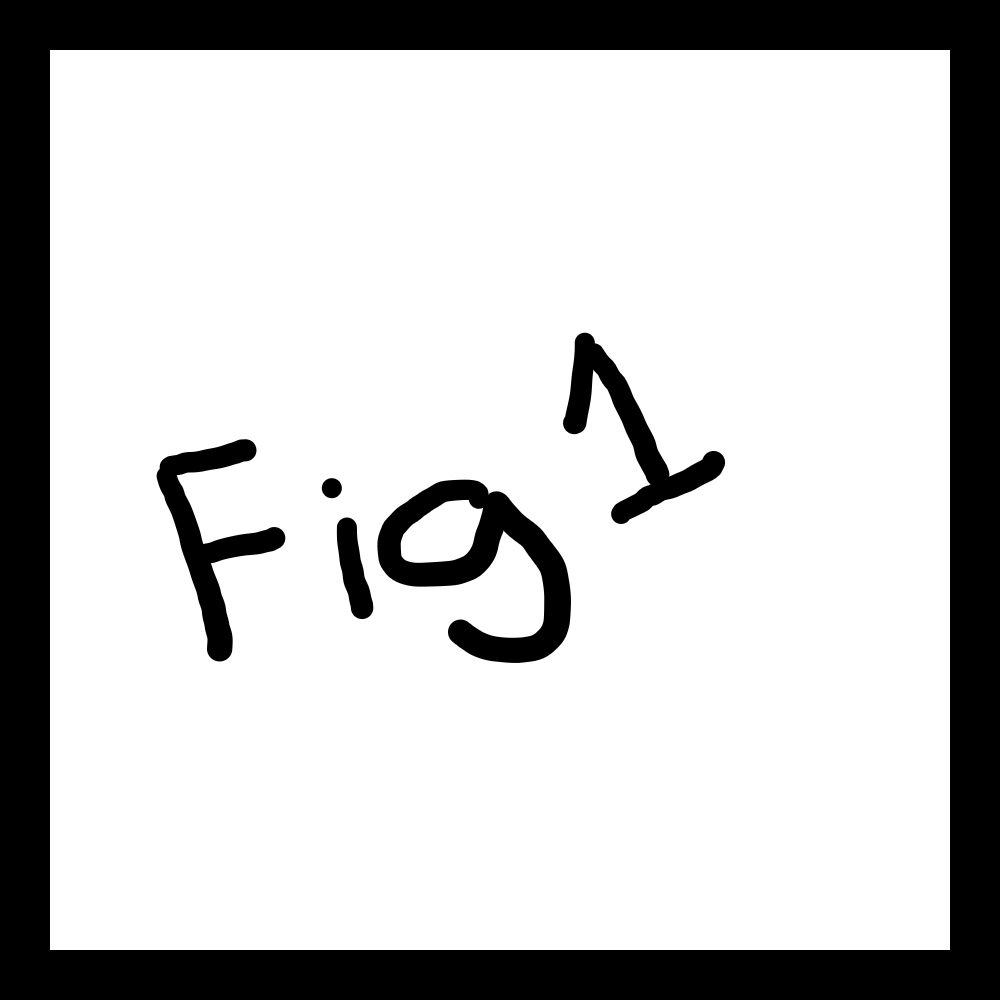
\includegraphics[width=\textwidth,keepaspectratio]{Figures/ExampleFigure1.png}}
	\caption{Embed your graphics as pdf. Lovely vector graphics! If I see any jpeg text I am sad.}
	\label{fig:Example1}
\end{figure}

\begin{figure}
	\centering
	\centerline{
\includegraphics[width=\textwidth,keepaspectratio]{Figures/ExampleFigure2.png}}
	\caption{This is a caption.}
	\label{fig:Example2}
\end{figure}


%%%%%%%%%%%%%%%%%%%%%%%%%%%%%%%%%%%%%%%%%%%%%%%%%%%%%%%%%%%%%%%%%%%%%%%%%%%%%%%%%
\subsection{Equations}
This is an equation reference: \eqref{eq:myEq}.

\begin{equation} \label{eq:myEq}
    a =  \DIFdel{3
}  \DIFadd{2
} \end{equation}

where $a$ is a variable.


%%%%%%%%%%%%%%%%%%%%%%%%%%%%%%%%%%%%%%%%%%%%%%%%%%%%%%%%%%%%%%%%%%%%%%%%%%%%%%%%%
\subsection{Tables}
This is a table reference: \tbref{tb:myTable}.

This is a fairly basic table. See threeparttable if you want table notes (footnotes for tables).

\begin{table}[!h]
    \centering
    \begin{tabular}{llll}
        \hline
        & & \multicolumn{2}{l}{Measurement error}\\
        Measurement & Unit & Mean & Standard deviation\\
        \hline
        $x_n$ & mm &  \DIFdelFL{5.2 }  \DIFaddFL{3.5 } &  \DIFdelFL{8.6}  \DIFaddFL{7.2} \\
        $y_n$ & mm &  \DIFdelFL{3.5 }  \DIFaddFL{5.1 } & 3.0\\
        $z_n$ & mm & -6.5 & 9.1\\
        $\theta_q$ & degrees & 1.6$\degree$ & 2.9$\degree$\\
        \hline
        \end{tabular}
    \caption{Average measurement error over all  \DIFdelFL{99 successful }  \DIFaddFL{200 } measurements. $(x_n, y_n, z_n)$ are defined somewhere else. $\theta_q$ is the rotational misalignment as a quaternion angular distance.}
    \label{tb:myTable}
\end{table}


%%%%%%%%%%%%%%%%%%%%%%%%%%%%%%%%%%%%%%%%%%%%%%%%%%%%%%%%%%%%%%%%%%%%%%%%%%%%%%%%%
%%%%%%%%%%%%%%%%%%%%%%%%%%%%%%%%%%%%%%%%%%%%%%%%%%%%%%%%%%%%%%%%%%%%%%%%%%%%%%%%%
\section{Conclusions and Future Work} \label{sec:conclusions}
Thus ends the example manuscript.

 \DIFdel{I can't be bothered to recommend future work }  \DIFadd{Recommend future work is to add the function of the powershell scripts into latexdiff itself} .


\FloatBarrier
%%%%%%%%%%%%%%%%%%%%%%%%%%%%%%%%%%%%%%%%%%%%%%%%%%%%%%%%%%%%%%%%%%%%%%%%%%%%%%%%%
%%%%%%%%%%%%%%%%%%%%%%%%%%%%%%%%%%%%%%%%%%%%%%%%%%%%%%%%%%%%%%%%%%%%%%%%%%%%%%%%%
\bibliographystyle{elsarticle-num}
\bibliography{Bibliography/Bibliography.bib}

%%%%%%%%%%%%%%%%%%%%%%%%%%%%%%%%%%%%%%%%%%%%%%%%%%%%%%%%%%%%%%%%%%%%%%%%%%%%%%%%%
%%%%%%%%%%%%%%%%%%%%%%%%%%%%%%%%%%%%%%%%%%%%%%%%%%%%%%%%%%%%%%%%%%%%%%%%%%%%%%%%%
\end{document}
\endinput

